Medical named entity recognition and normalization (MER and MEN) are hierarchical tasks and their outputs potentially have mutual benefits for each other as well. Specifically, the output of MER, such as ``B-DISEASE", is a clear signal indicating the beginning of a disease entity, leading to reducing the searching space of MEN and vice versa. Therefore, we propose to incorporate two explicit feedback strategies into multi-task learning framework to model mutual enhancement effects between tasks~\footnote{Our code is at GitHub (https://github.com/SendongZhao/Multi-Task-Learning-for-MER-and-MEN).}.
 In addition, we exploit Bi-LSTM to power the sequential modeling of the text and CNN to encode clues hidden in character-level features such as \textbf{Zo}lmitriptan, \textbf{Zomig} and \textbf{Zomig}on.

\textbf{Notation.} We use $\mathbf{x}_{1:n}$ to denote a sequence of $n$ vectors $\mathbf{x}_1,..., \mathbf{x}_n$. $F_{\theta}(\cdot)$ is a Bi-LSTM parameterized with parameters $\theta$. We use $F_L(\cdot)$ as a forward LSTM and $F_R(\cdot)$ as a backward LSTM with specific sets of parameters $\theta_L$ and $\theta_R$. $MER(w_{1:n},i)$ is the function to represent medical named entity recognition taking word sequence $w_{1:n}$ and index $i$ as input and output the corresponding named entity tag $y_{MER}^{i}$. $MEN(w_{1:n},i)$ is the function to represent medical named entity normalization taking word sequence $w_{1:n}$ and index $i$ as input and output the corresponding controlled vocabulary tag $y_{MEN}^{i}$.
We use $\circ$ to denote a vector concatenation operation. $\mathbf{U}$ and $\mathbf{V}$ are matrices to map the feedback of one task to the other. In this paper, we denote scalars by lowercase letters, such as $x$; vectors by boldface lowercase letters, such as $\mathbf{x}$; and matrices by boldface uppercase letters, such as $\mathbf{X}$.

\subsection{CNN for Character-level Representation}
Previous studies~\cite{TACL792} have shown that CNN is an effective approach to extract morphological
information (like the prefix or suffix of a word) from characters of words and encode it into neural representations. Figure~\ref{fig: cnn} shows the CNN we use to extract character-level representation of a given word. The CNN is similar to the one in~\citeauthor{TACL792} (\citeyear{TACL792}) except that we use only character embeddings as the inputs to CNN, without character type features. A dropout layer is applied before character embeddings are fed into CNN.
\begin{figure}[h]
	\centering
	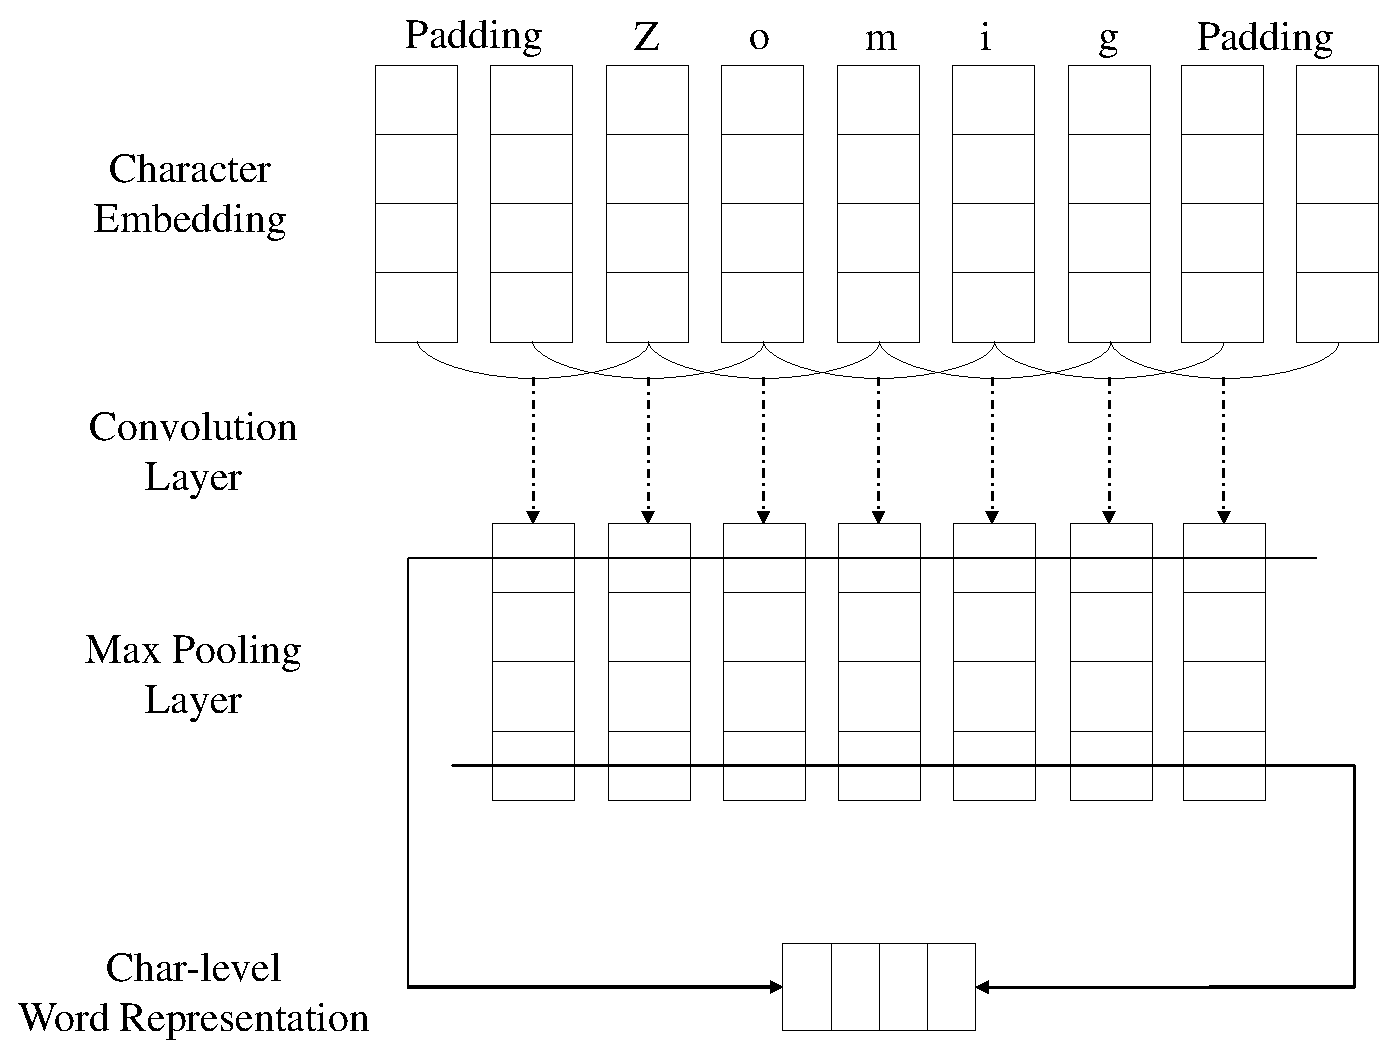
\includegraphics[width=0.45\textwidth]{fig/CNN}
	\vspace{-0.1in}	
	\caption{The CNN layer for extracting character-level word representation of word \textit{Zomig} (another name of the \textsc{Drug} \textit{Zolmitriptan} and \textit{Zomigon}).
		Dashed arrows indicate a dropout layer applied before character embeddings are fed into CNN. }\label{fig: cnn}
	\vspace{-0.15in}	
\end{figure}


\subsection{Sequence-labeling with Bi-LSTM}

The extracted features of each word, including pre-trained word embeddings from Word2Vec and character-level word representation from CNN, are fed into a forward LSTM and a backward LSTM. The output of each network at each time step is decoded by a linear layer and a log-softmax layer into log-probabilities for each tag category. These two vectors are then simply added together to produce the final output.

\begin{figure*}[tp]
	\centering
	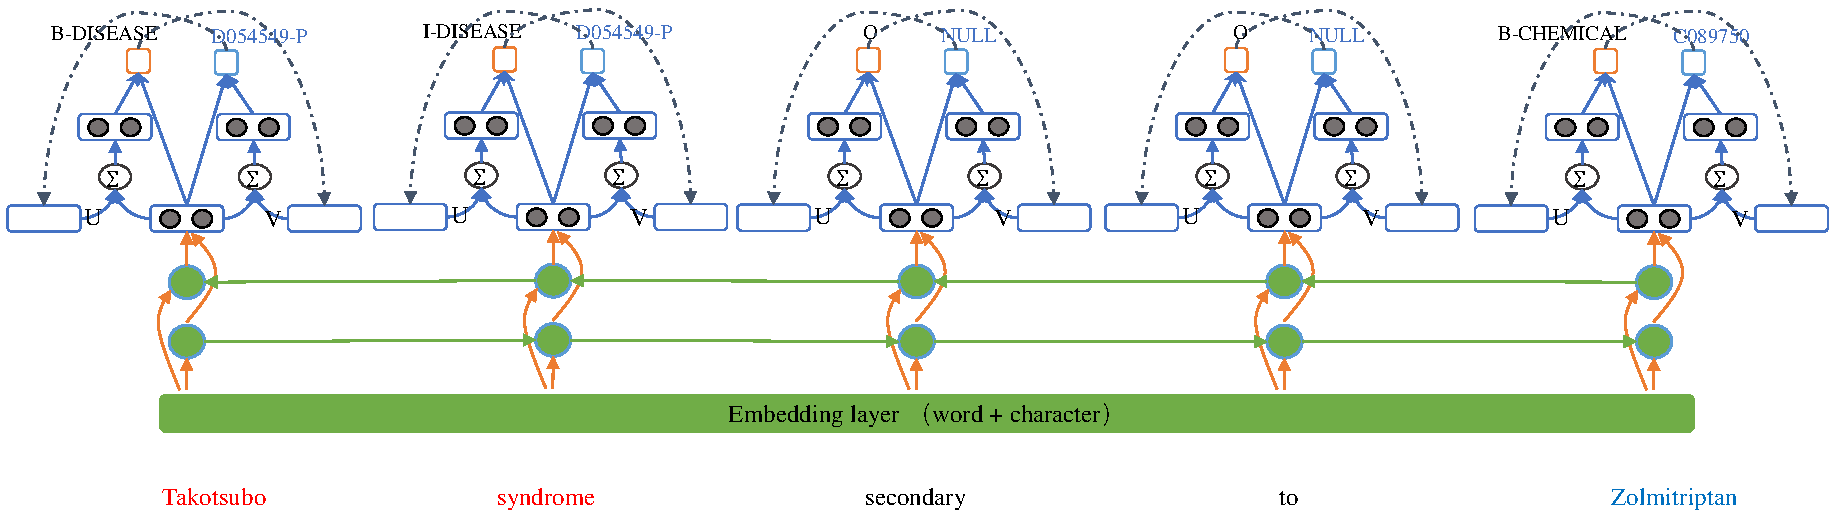
\includegraphics[width=0.95\textwidth]{fig/model}
	\vspace{-0.1in}	
	\caption{The main architecture of our neural
		multi-task learning model with two explicit feedback strategies for MER and MEN. The character embedding is computed by CNN in Figure~\ref{fig: cnn}.  Then
		the character representation vector is concatenated
		with the word embedding before feeding into the
		Bi-LSTM. Dashed arrows from the left to the  right is the feedback from MER to MEN.  Dashed arrows from the right to the left is the feedback from MEN to MER. Orange arrows indicate dropout
		layers applied on both the input and output vectors
		of Bi-LSTM. }\label{fig: model}
	\vspace{-0.15in}	
\end{figure*}

We view LSTM as a parameterized function $F_{\theta}(\mathbf{x}_{1:n})$ mapping a sequence of $n$ input vectors $\mathbf{x}_{1:n}$, $\mathbf{x}_i\in \mathbb{R}^{d_{in}} $ to output $n$ vectors $\mathbf{h}_{1:n}$, $\mathbf{h}_i \in \mathbb{R}^{d_{out}}$.
A Bi-LSTM is composed of two LSTMs, denoted as functions $F_L$ and $F_R$. One reading the sequence in its regular order, and the other reading it in reverse. Concretely, given a sequence $\mathbf{x}_{1:n}$ and
a desired index $i$, the function $F_{\theta}(\mathbf{x}_{1:n},i)$
is defined as:
\begin{equation*}
\begin{split}
F_{\theta}(\mathbf{x}_{1:n},i) = \mathbf{v}_i = \mathbf{h}_{L,i}\circ \mathbf{h}_{R,i}\\
\mathbf{h}_{L,i} = F_L(\mathbf{x}_1, \mathbf{x}_2, ..., \mathbf{x}_i)\\
\mathbf{h}_{R,i} = F_R(\mathbf{x}_n, \mathbf{x}_{n-1}, ..., \mathbf{x}_i)
\end{split}
\end{equation*}

The vector $\mathbf{v}_i = F_{\theta}(\mathbf{x}_{1:n},i)$ is then a representation of the $i$th item in $\mathbf{x}_{1:n}$, taking into account both the entire history $\mathbf{x}_{1:i}$ and the entire future $\mathbf{x}_{i:n}$.
Finally, in a deep Bi-LSTM, both $F_L$ and $F_R$ are k-layer LSTMs, and $F_{\theta}^{\ell}(\mathbf{x}_{1:n},i)= \mathbf{v}_i = \mathbf{h}_{L,i}^{\ell}\circ \mathbf{h}_{R,i}^{\ell}$.

In a sequence tagging task, we are given an input $w_1, ..., w_n$ and need to predict an output
$y_1, ..., y_n$, $y_i \in \mathbf{y}_{1:|L|}^i$, where $L$ is a label set of interest; i.e., in a medical named entity recognition task, $L$ is
the named entity tag set, and $y_i$ is the named entity tag for
word $w_i$ such as ``B-DISEASE".

If we take the inputs $\mathbf{x}_{1:n}$ to represent a sequence of sentence words $w_1, ..., w_n$, we can think of $\mathbf{v}_i = F_{\theta}(\mathbf{x}_{1:n}, i)$ as inducing an infinite window around a focus word $w_i$. We can then use $\mathbf{v}_i$ as an input to a multi-class classification function $f(\mathbf{v}_i)$, to assign a tag $\hat{y_i}$ to each input location $i$. The tagger is greedy: the tagging decisions are independent of each other. Alternatively, we can also feed the output vectors
of Bi-LSTM to the CRF layer to jointly decode the best tag sequence. Note that dropout layers are applied on both the input and output vectors of Bi-LSTM.

%However, as shown below and in other recent work using Bi-LSTM for sequence tagging, we can still produce competitive tagging accuracies, because of the richness of the representation $\mathbf{v}_i$ that takes the entire input sequence into account.

For a k-layer Bi-LSTM tagger for MER and MEN we get:
\begin{equation*}
\begin{split}
MER(w_{1:n},i)& = y_{MER}^{i}= \arg\max\mathbf{y}_{MER}^{i}\\
%&= \arg\max\mathbf{y}_{MER}^{i}\\
& = f_{MER}(\mathbf{v}_i^k)\\
MEN(w_{1:n},i) &=y_{MEN}^{i}= \arg\max\mathbf{y}_{MEN}^{i}\\
%&= \arg\max\mathbf{y}_{MEN}^{i}\\
& = f_{MEN}(\mathbf{v}_i^k)\\
\end{split}
\end{equation*}
\vspace{-0.2in}
\begin{equation*}
\begin{split}
&\mathbf{v}_i^k = F_{\theta}^k(\mathbf{x}_{1:n},i)\\
&\mathbf{x}_{1:n} = E(w_1), E(w_2), ..., E(w_n)
\end{split}
\end{equation*}
where $E$ as an embedding function mapping each
word in the vocabulary into a d-dimensional
vector, $\mathbf{y}_{MER}^{i}$ is the log-probabilities vector with the length of MER tag space, $y_{MER}^{i}$ is the output tag of MER, $\mathbf{y}_{MEN}^{i}$ is the log-probabilities vector with the length of MEN tag space, $y_{MEN}^{i}$ is the output tag of MEN, 
and $\mathbf{v}_i^k$ is the output of the $k$th Bi-LSTM layer
as defined above. All the parameters are trained separately for MER and MEN because we model MER and MEN as different sequence labeling tasks.

\subsection{Multi-task Mode with Explicit Feedback Strategies}
The dependencies between MER and MEN inspire us to explore their potential mutual benefits.
In order to make the most of the mutual benefits between MER and MEN, we propose to feed the above mentioned Bi-LSTM and its variants into multi-task learning framework with two explicit feedback strategies, as shown in Figure~\ref{fig: model}. This method (1) is able to convert hierarchical tasks into parallel multi-task mode while maintaining mutual supports between tasks; (2) benefits from general representations of both tasks provided by multi-task learning; (3) is effective in determining boundaries of medical named entities through explicit feedback strategies thus improves the performance of both MER and MEN.

We experiment with a multi-task learning architecture based on stacked Bi-LSTM, CNNs and CRF. Multi-task learning can be seen as a way of regularizing model induction by sharing representations with other inductions. We use stacked Bi-LSTM-CNNs-CRF with task supervision from multiple tasks, sharing Bi-LSTM-CNNs layers among the tasks.

MER and MEN are hierarchical tasks and their outputs potentially have mutual benefits for each other as well. It means MEN can take MER results as input, while the results of MEN can be also useful for MER. However, MER and MEN can be implemented independently as different sequence tagging tasks.  
Therefore, we 1) follow the popular strategy of multi-task learning to share representations between MER and MEN; and 2) propose to use mutual feedback between MER and MEN, i.e., the result of MER is fed into the MEN as part of the input and the result of MEN is fed into the MER as part of the input. The multi-task learning with two explicit feedback strategies for MER and MEN is defined as:
\begin{equation*}
\begin{split}
MER(w_{1:n},i) &= y_{MER}^{i}=\arg\max\mathbf{y}_{MER}^{i}\\
&= f_{MER}(\mathbf{v}_i^{MER})\\
MEN(w_{1:n},i) &= y_{MEN}^{i}=\arg\max\mathbf{y}_{MEN}^{i}\\
& = f_{MEN}(\mathbf{v}_i^{MEN})\\
\end{split}
\end{equation*}
\vspace{-0.1in}
\begin{equation*}
\begin{split}
&\mathbf{v}_i^{MER} = \mathbf{v}_i^k \circ (\mathbf{v}_i^k+\mathbf{y}_{MEN}^{i}\mathbf{U})\\
%&\mathbf{v}_i^{MER} = \mathbf{v}_i^k \circ \mathbf{y}_{MEN}^{i}\mathbf{U}\\
&\mathbf{v}_i^{MEN} = \mathbf{v}_i^k \circ  (\mathbf{v}_i^k+\mathbf{y}_{MER}^{i}\mathbf{V})\\
%&\mathbf{v}_i^{MEN} = \mathbf{v}_i^k \circ  \mathbf{y}_{MER}^{i}\mathbf{V}\\
&\mathbf{v}_i^k = F_{\theta}^k(\mathbf{x}_{1:n},i)\\
&\mathbf{x}_{1:n} = E(w_1), E(w_2), ..., E(w_n)
\end{split}
\end{equation*}
where $f_{MER}(\mathbf{v}_i^{MER})$ is the MER multi-class classification function and $f_{MEN}(\mathbf{v}_i^{MEN})$ the MEN multi-class classification function. $\mathbf{v}_i^{MER}$ is the input of MER multi-class classification function, which combines the output of the shared stacked Bi-LSTM-CNNs and the explicit feedback from MEN.  $\mathbf{v}_i^{MEN}$ is the input of MEN multi-class classification function, which combines the output of the shared Bi-LSTM-CNNs and the explicit feedback from MER. $\mathbf{U}$ is the matrix to map the feedback from MEN to MER, $\mathbf{V}$ maps the  feedback from MER to MEN. You can consider $(\mathbf{v}_i^k+\mathbf{y}_{MER}^{i}\mathbf{V})$ as a modification according to the feedback from MER, which could make $\mathbf{v}_i^k$ a better vector to get the correct label, the same as $\mathbf{v}_i^k+\mathbf{y}_{MEN}^{i}\mathbf{U}$.

In the multi-task learning setting, we have two prediction tasks over the same input vocabulary space. These two prediction tasks share k-layer Bi-LSTM-CNNs (i.e., hard parameter sharing). Each task has
its own output vocabulary (a task-specific tag set), but all of them map the length $n$ input sequence into a length $n$ output tag sequence.

\textbf{The Multi-task training protocol.} 
We assume to separate training set into $T$ different subsets corresponding to $T$ different tasks. We label $T$ different subsets as  $D_1, ..., D_T$, where
each $D_t$ contains pairs of input-output sequences ($w_{1:n}$, $y_{1:n}^t$), $w_i \in W$, $y_i^t \in L^t$. The input sets of words $W$ is shared across tasks, but the output sets (tag set) $L^t$ are task dependent.

At each step in the training process we choose a random task $t$, followed by a random training instance $(w_{1:n}, y_{1:n}^t)\in D_t$. We use the tagger of task $t$ to predict the labels $\hat{y}_i^t$, suffer a loss with respect to the true labels $y_i^t$ and update the output log-probabilities vector $\mathbf{y}_i^t$ of $w_{1:n}$ as well as the model parameters. 
If we choose MER at the very first step, we take the feedback from MEN as a log-probabilities vector with the initialization of each element having the same value $\frac{1}{|L^t|}$ and vice versa, where $|L^t|$ is the length of the tag set of task $t$.
Notice that a task $t$ (eg. MER and MEN in this paper) is associated with the stacked Bi-LSTM-CNNs. The update for a sample from task $t$ affects the parameters of $f_t$ and the shared $k$-layer functions $F_{\theta}^1, .., F_{\theta}^k$, but not the parameters of $f_{{t}'\neq t}$.
This asynchronous training protocol makes it possible to implement our model in distributed way.
We tried a synchronized way of training as well but did not lead to any difference in results. 
